6. \begin{figure}[ht!]
\center{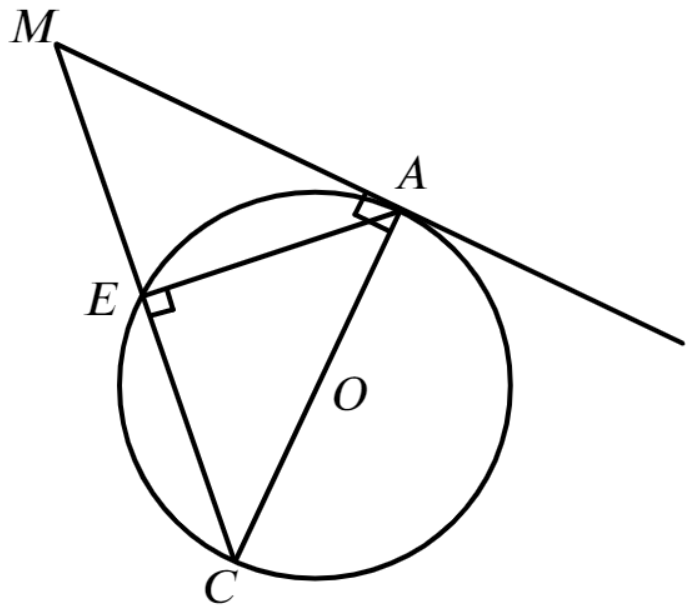
\includegraphics[scale=0.35]{g9-6.png}}
\end{figure}\\
Угол $AEC$ опирается на диаметр $AC,$ а $\angle MAC$ --- угол между радиусом и касательной, значит они равны $90^\circ.$ Тогда $MAC$ является прямоугольным треугольником, а $AE$ --- его высота. Найдём $MC=\sqrt{MA^2+AC^2}=\sqrt{25+144}=13$ и посчитаем его площадь двумя способами: $S=\cfrac{5\cdot12}{2}=\cfrac{AE\cdot13}{2},$ значит $AE=\cfrac{60}{13}.$\\
